\clearpage
\section{Configuring ROS for mapping}

During the installation of ROS on Ubuntu a new package named Hector-slam was discovered.
This package allows ROS to generate a map without the use of the GMapping package, which was one of the packages that caused issue during the installation process on Raspbian. Its biggest advantage is that it does not rely on odometry to know whether the reference frame has changed.
%TODO: we talk about Hector slam here, but we already mentioned it before.

\subsection{How ROS works}
During our development, we gained a deep understanding of how all the moving parts in ROS work together.

\begin{figure}[H]
	\centering
	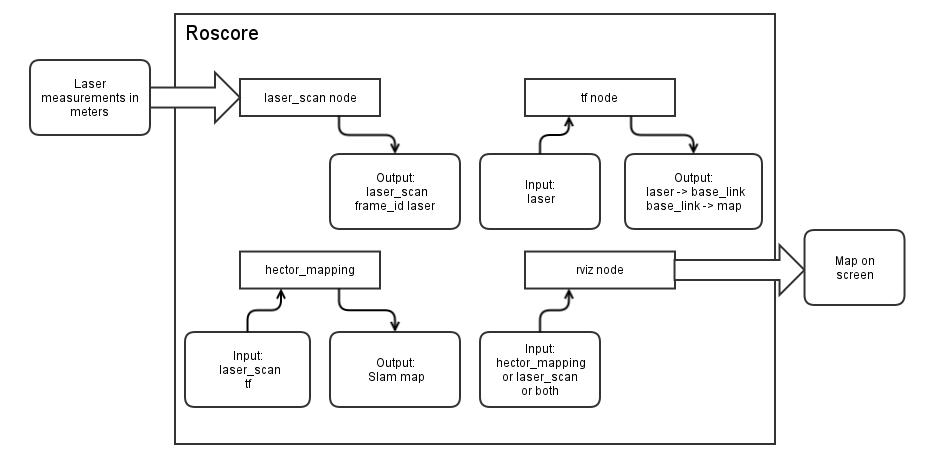
\includegraphics[width=1\linewidth]{images/ROSflow.png}
	\caption{Ros flow}
\end{figure}

Roscore is the main process behind ROS. It allows for all running nodes to talk to each other. By itself it does nothing.

Nodes are the smallest pieces of ROS that are put together to form a full application. They are run as separate applications, all with their own executable files. The only way nodes communicate is through the roscore. To make a node, it is necessary to use the ROS library in whatever programming language is desired.

Roslaunch is the ROS command that allows starting multiple nodes, and also allows giving parameters to nodes. Roslaunch executes nodes that are specified in an XML file you give it, called the launchfile.

%TODO: include our launchfile here

\subsection{something else}
%TODO: change subsection title
During this stage of testing, ROS gathers the data and generates the map directly on the Raspberry Pi. The Raspberry Pi is accessed through SSH and the generated map is then broadcast to computer through the SSH connection.

%TODO: Talk about SSHing into ROS here - Anthony will do that.

\begin{figure}[H]
	\centering
	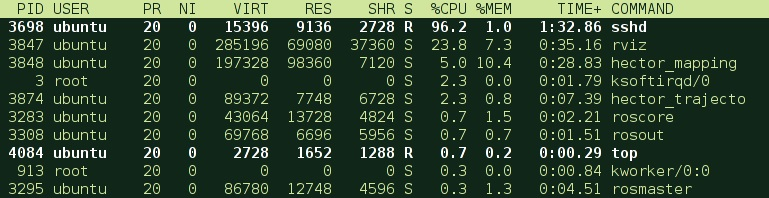
\includegraphics[width=.8\linewidth]{images/rvisScreenshotCropped.jpg}
	\caption{The resource usage}
\end{figure}


After testing the Hector SLAM some lag issues were experienced, which seemed to be caused by multiple things: One thing could be that generating the map on the actual Raspberry Pi required too many resources from the CPU, another could be that the transfer of the visualization to the computer screen required more bandwidth than there could be supplied.

To reduce the amount of resources used by the Raspberry Pi, the map needs to be generated and visualized using separate computing unit. ROS is built to have separate nodes with a main computing unit.

